\documentclass[aspectratio=169,xcolor=table,10pt, notes=hide]{beamer}


\usetheme[faculty=phil]{fibeamer}
\usepackage{polyglossia}

\setmainlanguage{russian} %% main locale instead of `english`, you
%% can typeset the presentation in either Czech or Slovak,
%% respectively.
\setotherlanguages{english} %% The additional keys allow
%%
%%   \begin{otherlanguage}{czech}   ... \end{otherlanguage}
%%   \begin{otherlanguage}{slovak}  ... \end{otherlanguage}
%%
%% These macros specify information about the presentation
\title[Theoretical Mechanics]{Theoretical Mechanics, Quiz 10: KIN ENERGY} %% that will be typeset on the
\subtitle{Change of Kinetic Energy of a System \\ \  \\ \  } %% title page.
\author{Oleg Bulichev}
%% These additional packages are used within the document:
\usepackage{ragged2e}  % `\justifying` text
\usepackage{booktabs}  % Tables
\usepackage{tabularx}
\usepackage{tikz}      % Diagrams
\usetikzlibrary{decorations.pathreplacing,calligraphy,calc,graphs, shapes, backgrounds}
\usepackage{amsmath, amssymb}
\usepackage{url}       % `\url`s
\usepackage{listings}  % Code listings
\usepackage{floatrow}
\usepackage{mathtools}
\usepackage{fontspec}
\usepackage{multicol}
\usepackage{pdfpages}
\usepackage{wrapfig}
\usepackage{animate}
\usepackage{booktabs}
\usepackage{multirow}
\usepackage{multimedia}
\usepackage{makecell}
\usepackage{colortbl}
\usepackage{hhline}
\usepackage{rotating}
\usepackage{amsmath}

\usepackage[font={}, labelfont=it,textfont={it},justification=centering, skip=0pt]{caption}
% will apply to all subcaptions
\usepackage[font={},skip=2pt]{subcaption}


\graphicspath{{resources/}}
\frenchspacing




% \setbeamertemplate{caption}[numbered]
\captionsetup[figure]{labelformat=empty}


\newcommand{\fbckg}[1]{\usebackgroundtemplate{\includegraphics[width=\paperwidth]{#1}}}%frame background

\usepackage[framemethod=TikZ]{mdframed}
\newcommand{\dbox}[1]{
\begin{mdframed}[roundcorner=3pt, backgroundcolor=yellow, linewidth=0]
\vspace{1mm}
{#1}
\vspace{1mm}
\end{mdframed}
}
\addtobeamertemplate{frametitle}{}{\vspace{-0.35cm}}

% \usepackage{pgfpages}
% \pgfpagesuselayout{4 on 1}[a4paper,border shrink=2mm,landscape]
\usepackage{color}
\usepackage{rotating}
\usepackage{tabularray}

\begin{document}
\setlength{\abovedisplayskip}{0pt}
\setlength{\belowdisplayskip}{0pt}
\setlength{\abovedisplayshortskip}{0pt}
\setlength{\belowdisplayshortskip}{0pt}

\fbckg{fibeamer/figs/title_page.png}
\frame[c]{\setcounter{framenumber}{0}
    \usebeamerfont{title}%
    \usebeamercolor[fg]{title}%
    \begin{minipage}[b][6.3\baselineskip][b]{\textwidth}%
        \textcolor{black}{\raggedright\inserttitle}
    \end{minipage}
    % \vskip-1.5\baselineskip

    \usebeamerfont{subtitle}%
    \usebeamercolor[fg]{framesubtitle}%
    \begin{minipage}[b][3\baselineskip][b]{\textwidth}
        \raggedright%
        \insertsubtitle%
    \end{minipage}
    \vskip.25\baselineskip
}

\note{}

\fbckg{fibeamer/figs/common.png}

\begin{frame}[t]{Quiz 10}
  \small
\begin{minipage}{0.6\textwidth}
  A homogeneous rod $OA$ of length $l$ and mass $M$ can rotate around a horizontal fixed axis $O$ passing through its end perpendicular to the plane of the figure. A coil spring, whose coefficient of elasticity is $c$, is attached at one end to the fixed axis $O$ and at the other end to the rod. The rod is at rest in a vertical position, and the spring is not deformed. 

\bigskip

What speed must be given to the end $A$ of the rod to make it deflect from the vertical by an angle equal to $60^\circ$?
\end{minipage}
\begin{minipage}{0.39\textwidth}
  \begin{figure}[H]
    \centering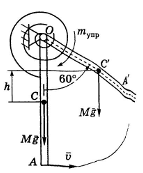
\includegraphics[height=4cm,width=1\textwidth,keepaspectratio]{quiz10_1}
    \caption*{Quiz 10, Task 1}
  \end{figure}
\end{minipage}
\end{frame}

\end{document}

